\chapter{Propagation Effects: Plasma, Dust, and Gravitational Lensing}
\label{chap:e21}

\begin{chapteropening}
Up to now we have almost always been asking the same kind of question: \textbf{what does the source really look like?}: its angular diameter, its coherence time, its photon statistics. But there is one thing we have quietly been assuming away: that as light sets out from the source and flies all the way to the telescope, the intervening thousands of light-years, the billions of light-years, are ``transparent.'' Of course they are not. Light must pass through tenuous free electrons, turbulent magnetized plasma, nebulae full of drifting dust grains, and even spacetime bent by massive objects. Every layer it crosses silently rewrites its arrival time, frequency, polarization, direction, and even ``how many copies it has.''

This chapter is about making clear ``what happens along the way.'' The through-line is as follows. First we treat propagation as a \textbf{channel with memory}, it does not simply multiply the signal by a constant, but refills every label carried by each photon. Then we take apart four classes of rewriters one by one: the \(\nu^{-2}\) dispersion of cold plasma (we will derive, without skipping a single step, ``why low-frequency photons arrive late''), the scattering and scintillation brought by turbulence, the extinction and reddening of dust, and the gravitational lensing of curved spacetime. Finally we return to the book's home turf: these effects both \textbf{contaminate} the signal (smearing out coherence, scrambling time stamps) and \textbf{encode} it (storing an electron ledger in the dispersion measure, storing cosmology in the time delay). It follows on from the bandwidth and coherence time of Chapter~\ref{chap:e02} and the time synchronization of Chapter~\ref{chap:e13}, and is the last processing step that translates ``source-end physics'' into ``detector events.''
\end{chapteropening}

\section{Treating propagation as a channel with memory}
\label{sec:e21-channel}

Let us set the scene. The easiest idea is to treat the medium as a piece of gray glass: light passes through, a little dimmer, a little redder, everything else unchanged. For average brightness and average color, this ``multiply by a constant'' picture is sometimes sufficient. But what this book cares about is the \textbf{event table} (Chapter~\ref{chap:e13}), each photon candidate carrying the labels of arrival time, frequency, polarization, and direction; and it also cares about \textbf{coherence}, the phase relations of the field between different times and different telescopes. For these quantities, ``gray glass'' is a catastrophic approximation, because what propagation really does is \textbf{rewrite the labels}: the frequency label determines how late it arrives, the polarization label is rotated by the magnetic field, the direction label is scattered apart and copied by the lens, and the arrival-time label is dragged out into echoes by multiple paths.

So a better first step is not to ask ``how bright was the source really,'' but to ask ``through what kind of channel must the source-end field pass to become an event on my detector.'' Writing it as a linear channel is the most direct. In the time domain, the electric field of the \(i\)-th observation channel (a given polarization, a given telescope, a given image, a given frequency channel) is the \textbf{convolutional superposition} of the source-end channel fields:
\begin{equation}
  E_{{\rm out},i}(t)
  =
  \sum_j\int h_{ij}(t-t')\,E_{{\rm src},j}(t')\,{\rm d}t'
  + n_i(t) .
  \label{eq:e21-channel-time}
\end{equation}
\begin{formulaexplain}
\(E_{{\rm out},i}\) is the field of the \(i\)-th observation channel, \(E_{{\rm src},j}\) is the field of the \(j\)-th source-end channel, \(h_{ij}\) is the response function from \(j\) to \(i\), and \(n_i\) is the foreground and detection noise. The integral sign is the key: propagation \textbf{has memory}: the light from one source-end instant is delayed and broadened to contribute to many observed instants.
\end{formulaexplain}
Symbol by symbol: \(i,j\) label polarization, telescope, image, or frequency channel (dimensionless indices); \(h_{ij}(t-t')\) is the impulse response, whose dimension depends on the field normalization, but what is truly useful are its three characteristics: the \textbf{time width} (how much the signal is broadened), the \textbf{peak delay} (how much the signal as a whole arrives late), and the \textbf{relative phase} between different channels; \(n_i(t)\) is the sum of foreground thermal radiation, airglow background, and detection-chain noise. If the medium only absorbs and does not scatter, \(h_{ij}\) is approximately a diagonal, amplitude-suppressed delta function; if there is Faraday rotation, it ``transfers funds'' between two linear polarization channels; if there is scattering or lensing, it simultaneously stirs together direction and arrival time. The barycentric correction, clock offsets, atmospheric delay, and instrumental electronic delay are also all part of this \(h_{ij}\): pulsar timing is precisely the most mature paradigm for taking these terms apart one by one down to the nanosecond level \citep{2006MNRAS.372.1549E}.

Translating back into the language of the event table: a photon candidate is a row \((t_q,\nu_q,p_q,\bm{x}_q,w_q)\): arrival time \(t_q\) (in s), frequency \(\nu_q\) (in Hz), polarization channel \(p_q\), spatial label \(\bm{x}_q\) (pixel, baseline, or telescope index), and quality weight \(w_q\). What remains to be done in this section is to write out a concrete form of that abstract \(h_{ij}\) in Equation~\eqref{eq:e21-channel-time} for each of the four classes of medium, seeing exactly how it modifies these five labels: dispersion modifies \(t_q(\nu_q)\), Faraday rotation modifies \(p_q(\lambda_q^2)\), scattering spreads the \(t_q\) of a narrow pulse into a long tail, dust modifies the probability that a given \(\lambda_q\) is received, and lensing copies one source event into several sets of \((\bm{x}_q,t_q)\).

Before beginning, let us spread the \textbf{map of orders of magnitude} out on the table, so that later, whenever we compute a number, we know where we stand. The dispersion measure (which we will define shortly) of the Galaxy toward high Galactic latitude is often \(30\text{--}100\,{\rm pc\,cm^{-3}}\), while fast radio bursts (FRBs) can reach \(10^{3}\text{--}10^{4}\,{\rm pc\,cm^{-3}}\). The rotation measure of the ordinary interstellar medium is mostly \(1\text{--}10^{2}\,{\rm rad\,m^{-2}}\), reaching \(10^{4}\text{--}10^{5}\,{\rm rad\,m^{-2}}\) in strongly magnetized dense environments. Scattering broadening ranges from microseconds to seconds, growing extremely fast at the low-frequency end. Optical extinction is often less than \(0.1\) magnitude at high Galactic latitude, and can reach several magnitudes in the Galactic disk and molecular clouds. The time delay of gravitational lensing spans the largest range: stellar-mass lenses give microseconds to milliseconds, and galaxy strong lensing is often days to years. Keep this map in mind, and every formula in this chapter can be pinned to a real number.

\section{Cold plasma dispersion: why low-frequency photons arrive late}
\label{sec:e21-dispersion}

Let us pick out the cleanest of the rewriters: cold plasma, that is, the tenuous free electrons pervading interstellar and intergalactic space. It has a very mild and very useful property: it does not randomize the pulse, but merely makes \textbf{low-frequency photons arrive slightly late}. And ``how late'' is precisely proportional to the total number of electrons encountered along the way. That is to say, dispersion is both a ``contaminant'' (it smears an instantaneous burst into a swept slanted line in frequency) and an ``encoder'' (the slope of that line is the electron ledger along the line of sight). We will derive this \(\nu^{-2}\) law without skipping a single step.

\paragraph{From refractive index to group velocity}
\label{sec:e21-groupvel}

The response of free electrons to an electromagnetic wave gives the refractive index of cold plasma. When the wave frequency is much higher than the plasma frequency (we will verify shortly that this condition holds for radio observation),
\begin{equation}
  n(\omega)\simeq 1-\frac{\omega_p^2}{2\omega^2},
  \qquad
  \omega_p^2=\frac{4\pi n_e e^2}{m_e}.
  \label{eq:e21-plasma-index}
\end{equation}
\begin{formulaexplain}
\(n(\omega)\) is the refractive index (dimensionless), \(\omega\) is the angular frequency, \(\omega_p\) is the plasma frequency, \(n_e\) is the free-electron number density, and \(e,m_e\) are the electron charge and mass (CGS units). The more electrons, the larger \(\omega_p\), and the more markedly a low-frequency wave deviates from vacuum propagation.
\end{formulaexplain}
Symbol by symbol: \(n_e\) is in \({\rm cm^{-3}}\), commonly \(10^{-2}\text{--}10^{-1}\,{\rm cm^{-3}}\) in the Galactic warm ionized medium and many orders of magnitude higher in HII regions and FRB host environments; \(\omega_p=\sqrt{4\pi n_e e^2/m_e}\) is the plasma's own natural oscillation frequency (in \({\rm rad\,s^{-1}}\)). Let us plug in a number to get a feel: taking \(n_e=0.03\,{\rm cm^{-3}}\), with the CGS values \(e=4.8\times10^{-10}\,{\rm esu}\), \(m_e=9.1\times10^{-28}\,{\rm g}\), gives \(\omega_p\approx 9.8\times10^{3}\,{\rm rad\,s^{-1}}\), corresponding to a frequency \(\nu_p=\omega_p/2\pi\approx1.5\,{\rm kHz}\). And radio observation is at \(\nu\sim10^{8}\text{--}10^{9}\,{\rm Hz}\), so \(\omega\gg\omega_p\) holds extremely amply, and keeping only the first order in \(\omega_p^2/\omega^2\) in Equation~\eqref{eq:e21-plasma-index} is entirely sufficient.

The crucial physics is that information (the pulse envelope) does not propagate at the phase velocity but at the \textbf{group velocity} \(v_g={\rm d}\omega/{\rm d}k\), as was stressed back in Chapter~\ref{chap:e02} when discussing wave packets. To compute \(v_g\), first write the dispersion relation \(k=n\omega/c\):
\[
  k=\frac{n\omega}{c}
   =\frac{\omega}{c}\left(1-\frac{\omega_p^2}{2\omega^2}\right)
   =\frac{\omega}{c}-\frac{\omega_p^2}{2c\,\omega}.
\]
Differentiating term by term with respect to \(\omega\) (using \({\rm d}(\omega^{-1})/{\rm d}\omega=-\omega^{-2}\) for the second term):
\[
  \frac{{\rm d}k}{{\rm d}\omega}
  =\frac{1}{c}-\frac{\omega_p^2}{2c}\cdot\left(-\frac{1}{\omega^2}\right)
  =\frac{1}{c}\left(1+\frac{\omega_p^2}{2\omega^2}\right).
\]
The group velocity is its reciprocal, expanded to first order using the geometric series \((1+x)^{-1}\approx1-x\) (because \(x=\omega_p^2/2\omega^2\ll1\)):
\[
  v_g=\frac{{\rm d}\omega}{{\rm d}k}
     =\frac{c}{1+\dfrac{\omega_p^2}{2\omega^2}}
     \approx c\left(1-\frac{\omega_p^2}{2\omega^2}\right).
\]
This step already lets us ``see'' the physics: \(v_g<c\), and \textbf{the lower the frequency (the smaller \(\omega\)), the larger \(\omega_p^2/2\omega^2\), and the slower the group velocity}. Slow means arriving late. The root cause of low-frequency photons arriving late is this one line.

\paragraph{Summing up the delay along the line of sight}
\label{sec:e21-dmderive}

Now let us translate ``slow'' into ``how late.'' A path segment \({\rm d}l\) takes a time \({\rm d}l/v_g\); integrating along the whole line of sight:
\[
  t=\int\frac{{\rm d}l}{v_g}
   =\int\frac{1}{c}\left(1+\frac{\omega_p^2}{2\omega^2}\right){\rm d}l
   =\underbrace{\frac{L}{c}}_{\text{vacuum flight}}
   +\underbrace{\frac{1}{2c\,\omega^2}\int\omega_p^2\,{\rm d}l}_{\text{extra dispersive delay}} .
\]
The first term is the time for light to fly the whole path \(L\) in vacuum, independent of frequency, and observationally only a total zero point that cannot be measured. What can truly be measured is the second term: it is the \textbf{frequency-dependent} lateness. Substituting \(\omega_p^2=4\pi n_e e^2/m_e\), and noting that \(4\pi e^2/m_e\) is a constant that can be pulled outside the integral:
\[
  \Delta t
  =\frac{1}{2c\,\omega^2}\int\frac{4\pi n_e e^2}{m_e}\,{\rm d}l
  =\frac{2\pi e^2}{m_e c\,\omega^2}\int n_e\,{\rm d}l .
\]
Finally, using \(\omega=2\pi\nu\), i.e.\ \(\omega^2=4\pi^2\nu^2\):
\begin{equation}
  \Delta t
  =\frac{e^2}{2\pi m_e c}\,\frac{1}{\nu^2}\int n_e\,{\rm d}l
  \equiv \frac{e^2}{2\pi m_e c}\,\frac{{\rm DM}}{\nu^2},
  \qquad
  {\rm DM}\equiv\int n_e\,{\rm d}l .
  \label{eq:e21-dm-delay}
\end{equation}
\begin{formulaexplain}
\(\Delta t\) is the extra delay relative to vacuum, \(\nu\) is the observing frequency, and DM is the \textbf{dispersion measure}, i.e.\ the column density of free electrons along the line of sight \(\int n_e\,{\rm d}l\). The skeleton of the whole expression is \(\Delta t\propto {\rm DM}/\nu^{2}\): the lateness is proportional to the total number of electrons along the way and inversely proportional to the square of the frequency.
\end{formulaexplain}
This expression makes three things clear at once. First, \(\Delta t\propto\nu^{-2}\): this is the quantitative version of ``low frequency arrives late,'' and we derived it all the way from the group velocity with no skipped steps. Second, the constant out front, \(e^2/(2\pi m_e c)\), is a pure physical constant (in CGS); substituting the astronomer's customary pc for the path element \({\rm d}l\) of DM and GHz for the frequency, the delay difference between two frequency channels is the one every astronomer knows by heart:
\begin{equation}
  \Delta t_{\rm DM}
  =
  4.148808\,{\rm ms}\;
  \frac{{\rm DM}}{{\rm pc\,cm^{-3}}}
  \left[
  \left(\frac{\nu_1}{\rm GHz}\right)^{-2}
  -
  \left(\frac{\nu_2}{\rm GHz}\right)^{-2}
  \right].
  \label{eq:e21-dispersion-delay}
\end{equation}
\begin{formulaexplain}
\(\Delta t_{\rm DM}\) is the arrival-time difference between the two channels at frequencies \(\nu_1\) and \(\nu_2\). The coefficient \(4.148808\,{\rm ms}\) is just the value of the physical constant in Equation~\eqref{eq:e21-dm-delay} after converting to pc, \({\rm cm^{-3}}\), and GHz. The \(\nu_1^{-2}\) term for the low frequency (\(\nu_1<\nu_2\)) is larger, so the low-frequency channel arrives late, and what one sees in the dynamic spectrum is that swept trajectory bending down and to the right.
\end{formulaexplain}
Third, DM is a \textbf{column density, not a local density}: it cares only about how many electrons there are in total along the way, not about how they are distributed. Its unit is \({\rm pc\,cm^{-3}}\) (the length pc multiplied by the number density \({\rm cm^{-3}}\)).

Let us plug in a real number. Take \({\rm DM}=300\,{\rm pc\,cm^{-3}}\) (a typical value for a moderate-distance pulsar), \(\nu_1=0.6\,{\rm GHz}\), \(\nu_2=1.4\,{\rm GHz}\):
\[
  \Delta t_{\rm DM}=4.148808\times300\times\left(0.6^{-2}-1.4^{-2}\right)\,{\rm ms}
  \approx 1244.6\times(2.778-0.510)\,{\rm ms}\approx 2822\,{\rm ms}\approx 2.8\,{\rm s}.
\]
Nearly three seconds! From the same burst, the \(0.6\) GHz signal arrives almost three seconds later than the \(1.4\) GHz. Precisely for this reason, radio-pulse and FRB searches must first perform \textbf{de-dispersion} over a bank of trial dispersion measures (trial DMs), shifting each frequency channel back according to \(\nu^{-2}\) until the pulses in the different channels realign and the signal-to-noise spikes; the DM that maximizes the signal-to-noise is the measured value.

There is also an easily overlooked \textbf{contamination}: even if the overall de-dispersion is done correctly, each frequency channel itself has a finite bandwidth \(\Delta\nu\), and the delay difference between the high- and low-frequency ends within the channel has not been compensated, which smears the pulse wider:
\begin{equation}
  \Delta t_{\rm chan}
  \simeq
  8.3\,\mu{\rm s}\;
  \left(\frac{{\rm DM}}{{\rm pc\,cm^{-3}}}\right)
  \left(\frac{\Delta\nu}{\rm MHz}\right)
  \left(\frac{\nu}{\rm GHz}\right)^{-3}.
  \label{eq:e21-channel-smearing}
\end{equation}
\begin{formulaexplain}
\(\Delta t_{\rm chan}\) is the residual dispersive broadening within a finite-bandwidth channel, \(\Delta\nu\) is the channel bandwidth, and \(\nu\) is the channel center frequency. It is the result of differentiating Equation~\eqref{eq:e21-dispersion-delay} with respect to \(\nu\) and multiplying by \(\Delta\nu\), hence the \(\nu^{-3}\). The meaning: the higher the DM, the wider the channel, and the lower the frequency, the more easily microsecond-scale fine structure is washed flat.
\end{formulaexplain}
It is of one spirit with Chapter~\ref{chap:e02}: to obtain good time resolution, one must pay the price in bandwidth, only here the price is amplified by dispersion. For high-time-resolution astronomy, Equation~\eqref{eq:e21-channel-smearing} directly determines how finely the channels must be sliced.

\begin{figure}[tbp]
\centering
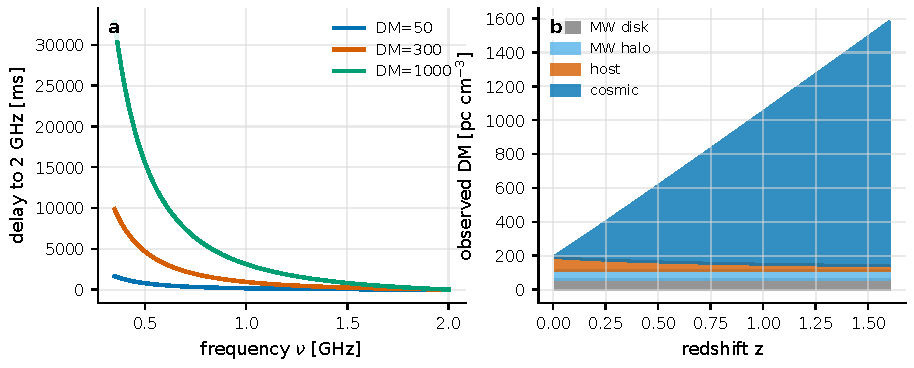
\includegraphics[width=0.94\linewidth]{figures/generated/chapter_14/ch14_dispersion_delay.pdf}
\caption{Cold-plasma dispersion and the FRB dispersion-measure budget. The left panel plots the arrival delay as a function of frequency (reference frequency \(2\,{\rm GHz}\)): the steep \(\nu^{-2}\) curve at the low-frequency end is why Equation~\eqref{eq:e21-dispersion-delay} makes DM so easy to read out from a broadband dynamic spectrum. The right panel breaks the observed dispersion measure of a nearby FRB into four parts: Galactic disk, Galactic halo, host galaxy, and cosmological plasma; the host term enters the observed value with a factor \((1+z)^{-1}\) because of cosmological time dilation.}
\label{fig:e21-dispersion}
\end{figure}

\paragraph{The dispersion measure as an electron ledger: from the Galaxy to cosmology}
\label{sec:e21-dmbudget}

Since DM is an electron ledger, one can conversely use it to measure electrons. But the ledger must sort out who owes what. The Galactic electron density is by no means constant: the NE2001 model stitches together the thick disk, thin disk, spiral arms, local bubble, and clumps, constraining the parameters with pulsar DMs, independent distances, and scattering data; YMW16 updated the thick disk, thin disk, spiral arms, Galactic center, and the treatment of the Magellanic Clouds/intergalactic medium, specifically to convert the \textbf{Galactic part of the DM} of a pulsar or an FRB into a distance or a foreground \citep{2002astro.ph..7156C,2017ApJ...835...29Y}. The Galactic-disk contribution of a high-Galactic-latitude line of sight is often \(30\text{--}100\,{\rm pc\,cm^{-3}}\), with the Galactic halo adding an order of \(50\text{--}100\,{\rm pc\,cm^{-3}}\); near the Galactic disk, an HII region, or a supernova remnant, local structure becomes more important than a smooth model.

For a cosmological FRB, the total observed dispersion measure is a bill spanning billions of light-years:
\begin{equation}
  {\rm DM}_{\rm FRB}
  =
  {\rm DM}_{\rm MW,ISM}
  +{\rm DM}_{\rm MW,halo}
  +{\rm DM}_{\rm cosmic}(z)
  +\frac{{\rm DM}_{\rm host}}{1+z} .
  \label{eq:e21-frb-dm-budget}
\end{equation}
\begin{formulaexplain}
The four terms are the contributions of the Galactic disk, the Galactic halo, the cosmological plasma along the way, and the host galaxy. The host term must be divided by \((1+z)\), because the frequency intervals and time intervals emitted at the host have already been stretched by a factor of the redshift by cosmic expansion en route to us. The same physical delay looks smaller to us.
\end{formulaexplain}
The physical meaning of each term: the first two come from our own Galaxy and can be subtracted using NE2001/YMW16; \({\rm DM}_{\rm cosmic}(z)\) is the baryonic electrons diffuse in the intergalactic medium, growing monotonically with redshift, and is the most valuable term in this expression; \({\rm DM}_{\rm host}\) is the host-galaxy contribution and is the hardest to constrain. Writing the cosmological term as an integral over a homogeneous universe:
\begin{equation}
  {\rm DM}_{\rm cosmic}(z)
  =
  \frac{3cH_0\Omega_b f_{\rm IGM}}{8\pi Gm_p}
  \int_0^z
  \frac{f_e(z')(1+z')}{\sqrt{\Omega_m(1+z')^3+\Omega_\Lambda}}
  \,{\rm d}z' .
  \label{eq:e21-cosmic-dm}
\end{equation}
\begin{formulaexplain}
\(\Omega_b,\Omega_m,\Omega_\Lambda\) are the baryon, matter, and dark-energy density parameters, \(H_0\) is the Hubble constant, \(m_p\) is the proton mass, \(f_{\rm IGM}\) is the fraction of baryons in the diffuse intergalactic medium, and \(f_e\) is the number of free electrons provided per baryon. The coefficient out front gives the mean baryon density, and the integrand describes how the electron number density and path length vary with redshift in an expanding universe.
\end{formulaexplain}
None of the components of this expression is mysterious: the coefficient \(3H_0^2\Omega_b/8\pi G\) is today's mean baryon mass density (the critical density times \(\Omega_b\)), divided by \(m_p\) to become a number density, then times \(f_e f_{\rm IGM}\) to give the electron number density; the \((1+z')\) in the integral is the net factor after the dilution of density by expansion is offset by the compression of the path, and the denominator \(\sqrt{\Omega_m(1+z')^3+\Omega_\Lambda}\) is the \(\Lambda\)CDM expansion rate \(H(z')/H_0\). There is one step here that must not be dropped: the line-of-sight element is not \({\rm d}l\) but rather \({\rm d}l=c\,{\rm d}z'/H(z')\) written in terms of redshift, which alone contributes a factor \(c/H_0\) (with \(H_0\) pulled out of \(H(z')=H_0\sqrt{\cdots}\) and placed in the denominator of the integrand). It is precisely this \(c/H_0\), merging with the \(H_0^2\) in the critical density, that turns the prefactor from the mass-density form ``\(3H_0^2\Omega_b/(8\pi G)\) divided by \(m_p\)'' into the \(3cH_0\Omega_b f_{\rm IGM}/(8\pi Gm_p)\) with \(cH_0\) in the expression, one factor of \(c/H_0\) more than the pure mass density. If the reader works through the algebra, do remember this share of \(c/H_0\) coming from \({\rm d}l=c\,{\rm d}z'/H(z')\), otherwise the prefactor will be off by a factor. Its physical meaning is astonishingly practical: \textbf{the DM--redshift relation of FRBs directly weighs how many baryons there are in the universe}: this was once the ``missing baryon'' problem, and today the relation given by FRB samples can already measure the cosmic baryon content. The true scatter comes from the inhomogeneity of the cosmic web, often written as \(\sigma_{\rm DM}\simeq F z^{-1/2}\), with \(F\sim0.1\text{--}0.4\) corresponding to different feedback and halo-gas distributions \citep{2020Natur.581..391M,2014ApJ...790..101S}. This is the most beautiful example of ``contamination becoming encoding'': dispersion was originally a fog standing in front of the source, and it turns out that this fog itself weighs the baryons of the universe.

\section{Faraday rotation: adding the direction of the magnetic field to dispersion}
\label{sec:e21-faraday}

Dispersion counts only the number of electrons and throws away the information of the magnetic field. If the plasma is \textbf{magnetized}, there is a second imprint: left- and right-handed circular polarizations have different phase velocities in a magnetized plasma, so the plane of vibration of linear polarization is rotated as it propagates, and the rotation angle is precisely proportional to the square of the wavelength:
\begin{equation}
  \psi(\lambda)=\psi_0+{\rm RM}\,\lambda^2 .
  \label{eq:e21-rm-angle}
\end{equation}
\begin{formulaexplain}
\(\psi\) is the observed linear polarization angle, \(\psi_0\) is the source's intrinsic polarization angle, \(\lambda\) is the wavelength, and RM is the \textbf{rotation measure}. The slope of the polarization angle against \(\lambda^2\) is RM. So as long as one measures the polarization angle at several frequencies and plots it as a \(\psi\)--\(\lambda^2\) diagram, the slope gives the cumulative effect of the magnetized plasma.
\end{formulaexplain}
It is a sister to dispersion: dispersion gives the arrival time a slope of \(\nu^{-2}\) (equivalent to \(\lambda^2\)), while Faraday gives the polarization angle a slope of \(\lambda^2\). Both are ``reading a slope.'' The rotation measure itself is the path integral of the electron density and the line-of-sight magnetic-field component:
\begin{equation}
  {\rm RM}
  =
  0.812
  \int
  \left(\frac{n_e}{{\rm cm^{-3}}}\right)
  \left(\frac{B_\parallel}{\mu{\rm G}}\right)
  \left(\frac{{\rm d}l}{\rm pc}\right)
  \;{\rm rad\,m^{-2}} .
  \label{eq:e21-rm-definition}
\end{equation}
\begin{formulaexplain}
\(B_\parallel\) is the magnetic-field component along the line of sight (toward the observer), in units of microgauss (\(\mu{\rm G}\)). The key difference between RM and DM: the integrand of DM is \(n_e\) (always positive, only accumulating), while the integrand of RM is \(n_e B_\parallel\) (signed, and a field reversal cancels). So RM carries the \textbf{direction} information of the magnetic field.
\end{formulaexplain}
Dividing the two gives an electron-weighted estimate of the line-of-sight-averaged magnetic field:
\begin{equation}
  \langle B_\parallel\rangle
  \simeq
  1.232\,\mu{\rm G}\;
  \frac{{\rm RM}/{\rm rad\,m^{-2}}}{{\rm DM}/{\rm pc\,cm^{-3}}}.
  \label{eq:e21-bfield-rm-dm}
\end{equation}
\begin{formulaexplain}
\(\langle B_\parallel\rangle\) is the mean line-of-sight magnetic field inferred from the ratio of RM to DM. The coefficient \(1.232\,\mu{\rm G}\) is just the ratio of the two numerical coefficients in Equation~\eqref{eq:e21-rm-definition} and the definition of DM. This ratio has a direct physical meaning only when RM and DM come from the \textbf{same segment of medium}.
\end{formulaexplain}
This is not a ``universally applicable'' magnetic-field measurement; when using it, one must watch two pitfalls closely. First, if RM comes mainly from a magnetized host galaxy while DM comes mainly from the intergalactic medium, the two are not the same path, and Equation~\eqref{eq:e21-bfield-rm-dm} will severely underestimate the local field. Second, if the field reverses along the line of sight, RM cancels while DM does not, and the ratio is likewise distorted. RM studies of galaxy clusters and intergalactic fields often combine this kind of degeneracy with X-ray gas density, radio halos, and RM grids of background sources to disentangle it \citep{2002ARA&A..40..319C}. In order of magnitude, the \(|{\rm RM}|\) of an ordinary interstellar line of sight is mostly \(1\text{--}10^2\,{\rm rad\,m^{-2}}\), which, together with \({\rm DM}\sim30\,{\rm pc\,cm^{-3}}\), gives \(\langle B_\parallel\rangle\) of order microgauss, precisely the typical strength of the Galactic interstellar magnetic field.

\begin{figure}[tbp]
\centering
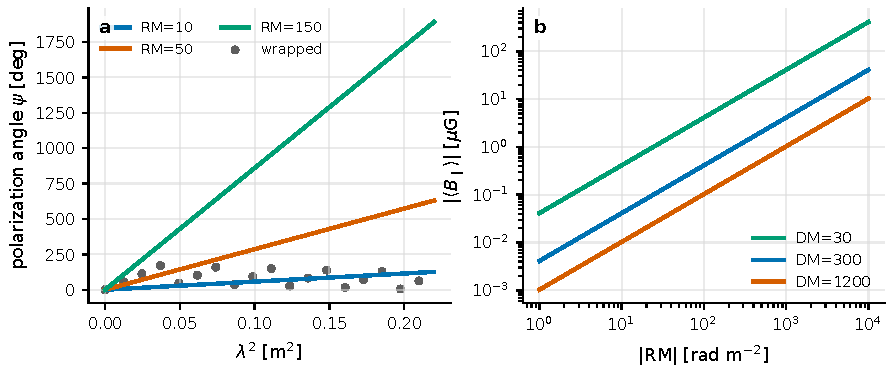
\includegraphics[width=0.94\linewidth]{figures/generated/chapter_14/ch14_faraday_rotation.pdf}
\caption{Two readings of Faraday rotation. The left panel is the linear relation \(\psi=\psi_0+{\rm RM}\,\lambda^2\); the black dots remind us that the polarization angle can only be measured modulo \(\pi\), and narrowband data easily suffer an \(n\pi\)-wrapping ambiguity (a sufficiently wide \(\lambda^2\) coverage is needed to fix a unique slope). The right panel plots \(\langle B_\parallel\rangle=1.232\,{\rm RM}/{\rm DM}\) as a function of RM: the same RM represents a stronger mean field in a tenuous, low-DM medium.}
\label{fig:e21-faraday}
\end{figure}

For coherence and polarization measurements, the implication of Faraday rotation is direct: if your receiving bandwidth spans a non-negligible range of \(\lambda^2\) and RM is large, then the polarization angles of different frequencies within the band are rotated to different directions, and averaging them without correction will \textbf{dilute} (depolarize) the net polarization: this is precisely the version, in the polarization dimension, of the spirit of Chapter~\ref{chap:e02}, ``phase misalignment within the bandwidth weakens coherent superposition.'' The remedy is to first measure RM, rotate the polarization angle of each channel back to its intrinsic value, and then superpose coherently.

\section{Scattering and scintillation: how multiple paths scramble coherence}
\label{sec:e21-scattering}

Both dispersion and Faraday rotation are very ``gentlemanly'': they only give different frequencies and different polarizations a definite relative delay or rotation, which is undone by removal. Scattering is different: it acts on the \textbf{direction} and on \textbf{coherence} itself. The interstellar electron density is not smooth, and turbulence stirs up density fluctuations on all scales; these fluctuations, like ground glass, crumple the flat wavefront. The consequences of the crumpling are threefold: the source image is angularly broadened (angular broadening), a narrow pulse is dragged out into a long tail (temporal broadening), and the intensity scintillates with time and frequency (scintillation): the three things are in fact one and the same thing projected onto angle, time, and frequency.

Let us first look at the temporal tail. After the wavefront is crumpled, light can reach us along many slightly longer paths, equivalent to an instantaneous signal at the source being spread over a short interval of time. In the simplest \textbf{single-thin-screen} approximation, the observed pulse is the convolution of the source pulse with an arrival-time kernel:
\begin{equation}
  I_{\rm obs}(t)
  =
  \int I_{\rm src}(t')\,P(t-t')\,{\rm d}t',
  \qquad
  P(t)=\frac{1}{\tau_{\rm sc}}\exp\!\left(-\frac{t}{\tau_{\rm sc}}\right)H(t).
  \label{eq:e21-scattering-convolution}
\end{equation}
\begin{formulaexplain}
\(I_{\rm obs}\) is the observed intensity, \(I_{\rm src}\) is the source-end intensity, \(P(t)\) is the scattering arrival-time kernel, \(\tau_{\rm sc}\) is the scattering broadening timescale, and \(H(t)\) is the step function. The kernel is a \textbf{one-sided} exponential: light can only be \textbf{delayed} by taking a detour, never arrive early, so a symmetric narrow pulse comes out as a ``steep-rise, slow-decay'' long tail.
\end{formulaexplain}
Here \(\tau_{\rm sc}\) is in seconds (or milliseconds), the \(1/e\) decay time of the long tail. A real line of sight may have multiple screens, anisotropic scattering, and a finite source size; the one-sided exponential is only the most commonly used low-order model. \(\tau_{\rm sc}\) depends strongly on frequency:
\begin{equation}
  \tau_{\rm sc}\propto \nu^{-\alpha}.
  \label{eq:e21-scattering-power}
\end{equation}
\begin{formulaexplain}
\(\alpha\) is the frequency index of scattering. Thin-screen theory for Kolmogorov turbulence gives \(\alpha\simeq4.4\), while the empirical average of multi-frequency pulsar samples is closer to \(3.9\pm0.2\). With so steep an index, going to lower frequency makes the scattering tail explode in length. This is the most troublesome enemy of low-frequency pulse searches.
\end{formulaexplain}
Empirically, a common fitting formula linking \(\tau_{\rm sc}\) to DM and frequency is used:
\begin{equation}
  \log_{10}\!\left(\frac{\tau_{\rm sc}}{{\rm ms}}\right)
  =
  -6.46
  +0.154\log_{10}{\rm DM}
  +1.07(\log_{10}{\rm DM})^2
  -3.86\log_{10}\!\left(\frac{\nu}{\rm GHz}\right),
  \label{eq:e21-bhat-scattering}
\end{equation}
\begin{formulaexplain}
This is an empirical scattering relation (DM in units of \({\rm pc\,cm^{-3}}\)), suitable only for order-of-magnitude estimates. The quadratic term \((\log_{10}{\rm DM})^2\) reflects high-DM lines of sight passing through more turbulence; \(-3.86\log_{10}\nu\) is the logarithmic version of Equation~\eqref{eq:e21-scattering-power}. The turbulent structure of a real line of sight brings a scatter far exceeding an order of magnitude.
\end{formulaexplain}
Plugging in numbers: at \({\rm DM}=300\,{\rm pc\,cm^{-3}}\), \(\nu=1.4\,{\rm GHz}\) it gives a broadening of order milliseconds; dropping to \(0.6\,{\rm GHz}\), by that \(\nu^{-3.86}\), the broadening grows to a dozen milliseconds or more. Scattering drags a millisecond pulse into a tens-of-milliseconds mush, and the microstructure is thereby lost: this is pure ``contamination.''

Now to the most crucial connection between this chapter and coherence. The temporal tail is, in the frequency domain, equivalent to a \textbf{decorrelation bandwidth} \(\Delta\nu_d\), the width over which the scintillation pattern still ``remembers itself'' in frequency:
\begin{equation}
  \tau_{\rm sc}\simeq \frac{C_1}{2\pi\,\Delta\nu_d}.
  \label{eq:e21-decorrelation-bandwidth}
\end{equation}
\begin{formulaexplain}
\(\Delta\nu_d\) is the decorrelation bandwidth of scintillation, and \(C_1\) is a constant related to the geometry and scattering spectrum (usually \(\sim1\)). It is the scattering version of the uncertainty relation ``time width is inversely proportional to spectral width'' of Chapter~\ref{chap:e02}: the longer the multipath delay (large \(\tau_{\rm sc}\)), the narrower the correlated bandwidth \(\Delta\nu_d\) in frequency.
\end{formulaexplain}
This expression lays bare the meaning of scattering for coherence measurement. Recall Chapter~\ref{chap:e02}: the coherence time \(\tau_c\simeq1/\Delta\nu\). Scattering is equivalent to superimposing an extra, random phase structure on the signal, whose ``coherence bandwidth'' is precisely \(\Delta\nu_d\). When scattering is strong and \(\Delta\nu_d\) is only a few tens of kHz, doing coherent superposition over a broadband of several hundred MHz amounts to forcing together thousands of mutually incoherent patches, the net coherence is diluted almost to zero. Conversely, scattering also \textbf{encodes} information: when scattering is weak and \(\Delta\nu_d\) is measurable, the drift of scintillation patches with time and frequency can be inverted for the velocity of the scattering screen, the distance from the screen to us, and even the angular size of the source, an ``interstellar scintillation telescope,'' whose effective angular resolution can reach microarcseconds, far surpassing any single-aperture telescope. These are the two faces of scattering: both the ground glass that smears out coherence, and a free ultra-high-resolution probe.

\begin{figure}[tbp]
\centering
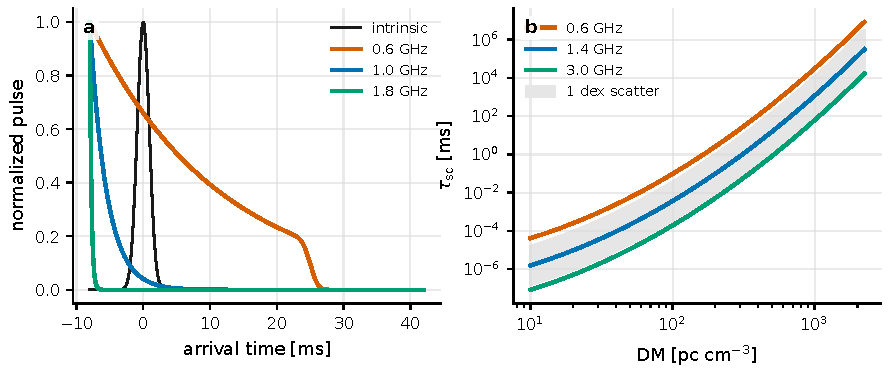
\includegraphics[width=0.94\linewidth]{figures/generated/chapter_14/ch14_scattering_broadening.pdf}
\caption{Interstellar scattering drags a short pulse into an arrival-time distribution with a long tail. The left panel convolves a narrow Gaussian pulse with a one-sided exponential kernel; the lower the frequency, the longer \(\tau_{\rm sc}\propto\nu^{-4}\) stretches the tail, and the symmetry of the pulse is utterly destroyed. The right panel uses the empirical relation to plot the variation of \(\tau_{\rm sc}\) with DM and frequency, with the gray band showing the common scatter of over an order of magnitude at fixed DM.}
\label{fig:e21-scattering}
\end{figure}

In passing: plasma does not only ``crumple'' the wavefront; a transverse gradient in the electron column density can also \textbf{refract} light like a (frequency-dependent) lens, with the low frequencies deflected more strongly, potentially causing narrowband magnification, caustics, or multiple images. This reminds us that even after the \(\nu^{-2}\) dispersion has been cleaned out, residual structure in the dynamic spectrum may still be a product of propagation rather than an intrinsic variation of the source \citep{1998ApJ...496..253C,2014MNRAS.437.2180E}. When doing millimeter-wave VLBI toward the Galactic center, this strong scattering screen is especially troublesome: to image the event-horizon scale of Sgr A*, one must simultaneously handle the intrinsic structure, the scattering blur, and the temporal variation \citep{2008Natur.455...78D,2022ApJ...930L..14E,2022ApJ...930L..15E}.

\section{Dust: a loss channel with wavelength selectivity}
\label{sec:e21-dust}

Plasma acts mainly on radio and arrival time; dust acts mainly on the optical and infrared \textbf{flux and color}. For optical photons, dust grains are like a picky loss channel: they absorb and scatter selectively by wavelength, with short waves (blue light) lost more than long waves (red light), so starlight passing through dust becomes both dimmer and redder. The most basic extinction relation is
\begin{equation}
  F_{\lambda,{\rm obs}}
  =
  F_{\lambda,{\rm int}}\,10^{-0.4A_\lambda},
  \label{eq:e21-extinction-flux}
\end{equation}
\begin{formulaexplain}
\(F_{\lambda,{\rm int}}\) is the intrinsic flux, \(F_{\lambda,{\rm obs}}\) is the extincted flux, and \(A_\lambda\) is the extinction at wavelength \(\lambda\), in magnitudes (mag). Magnitude is inherently a logarithmic scale, so \(A_\lambda\) suppresses the flux in the exponent in the form \(10^{-0.4A_\lambda}\): \(A_\lambda=1\) magnitude corresponds to the flux dropping to about \(0.40\) times, and \(A_\lambda=2.5\) to about \(0.10\) times.
\end{formulaexplain}
The variation of extinction with wavelength is summarized by two quantities that characterize its degree of ``reddening'':
\begin{equation}
  E(B-V)=A_B-A_V,
  \qquad
  R_V=\frac{A_V}{E(B-V)}.
  \label{eq:e21-rv-definition}
\end{equation}
\begin{formulaexplain}
\(E(B-V)\) is the difference in extinction between the blue band \(B\) and the visible band \(V\), called the \textbf{color excess}, measuring how much the starlight has been ``reddened''; \(R_V=A_V/E(B-V)\) is the ratio of total extinction to selective reddening, measuring the ``grayness'' of the extinction curve. The larger \(R_V\), the flatter (grayer) the curve, indicating that larger dust grains dominate.
\end{formulaexplain}
Term by term: \(A_B,A_V\) are the extinctions in the \(B\) and \(V\) bands (each in mag), and \(E(B-V)\) is also in mag. The Galactic mean is \(R_V\simeq3.1\), mostly \(2.5\text{--}3.5\) in the diffuse interstellar medium, and can reach above \(5\) in dense molecular clouds (large grains make the extinction grayer). The Cardelli--Clayton--Mathis (CCM) extinction law compresses the mean infrared, optical, and ultraviolet curves into a one-parameter family parameterized by \(R_V\); Fitzpatrick further pointed out that real lines of sight still have marked scatter, especially in the strength of the \(2175\,\text{\AA}\) ultraviolet bump (UV bump) and the far-ultraviolet upturn \citep{1989ApJ...345..245C,1999PASP..111...63F,2003ARA&A..41..241D}.

Here there is an \textbf{error floor} crucial for transient and polarization measurements. If you correct a blue source with \(E(B-V)=0.2\) magnitude using only a mean extinction law, a residual error of \(0.1\) magnitude at the ultraviolet end is nothing unusual, and for the polarization angle, the color temperature, and the early spectral energy distribution (SED) of a transient source, this is the dominant systematic error. In other words, dust not only dims the source, it also injects a non-negligible uncertainty into the measurement of ``color.''

Dust grains are mostly non-spherical, and they partly align their orientations in the interstellar magnetic field, so they absorb starlight of different vibration directions unequally, injecting a little \textbf{linear polarization} into the transmitted starlight. Its wavelength dependence is described by the empirical Serkowski relation:
\begin{equation}
  \frac{P(\lambda)}{P_{\max}}
  =
  \exp\!\left[-K\ln^2\!\left(\frac{\lambda_{\max}}{\lambda}\right)\right].
  \label{eq:e21-serkowski}
\end{equation}
\begin{formulaexplain}
\(P(\lambda)\) is the degree of linear polarization caused by dust, \(P_{\max}\) is the peak polarization, \(\lambda_{\max}\) is the peak wavelength, and \(K\) controls the curve width. It is a Gaussian-type peak in the variable \(\ln(\lambda_{\max}/\lambda)\): the polarization is maximal at \(\lambda_{\max}\) and decays symmetrically to both sides. The peak position \(\lambda_{\max}\) is sensitive to grain size.
\end{formulaexplain}
Empirically \(\lambda_{\max}\approx0.55\,\mu{\rm m}\), and the upper limit of the peak degree of polarization is about \(P_{\max}\lesssim9\,E(B-V)\%\) (i.e.\ at most about 0.9\% polarization per 0.1 mag of color excess). This upper limit is not reached on every line of sight; it is affected by grain shape, alignment efficiency, variations of the magnetic-field direction along the line of sight, and the superposition of multiple cloud layers \citep{1975ApJ...196..261S,2015ARA&A..53..501A}. For any experiment seeking to measure the source's intrinsic polarization, this dust polarization is a foreground that must be subtracted first.

Dust can also ``replay'' a brief burst as a \textbf{light echo} or an X-ray halo: the light of the burst is scattered into our line of sight by dust en route, and because it took a detour, it arrives later than the direct light. If the dust screen is located at a fraction \(x\) of the source-to-observer distance and the scattering angle is \(\theta\), the geometric delay is approximately
\begin{equation}
  \Delta t_{\rm dust}
  \simeq
  \frac{D_s}{2c}\,\frac{x}{1-x}\,\theta^2 .
  \label{eq:e21-dust-delay}
\end{equation}
\begin{formulaexplain}
\(\Delta t_{\rm dust}\) is the geometric delay of dust scattering, \(D_s\) is the source distance, \(x\) is the relative position of the dust screen (\(0\) at the source, \(1\) at the observer), and \(\theta\) is the scattering angle. The delay is proportional to \(\theta^2\), so an angularly resolved light echo can invert the geometric position of the dust: the expansion of the delay with scattering angle is a distance-measuring ruler.
\end{formulaexplain}
In order of magnitude, for a Galactic source an arcsecond-scale scattering angle gives a delay of hours to days; for an extragalactic source, the geometric position of the dust and the telescope angular resolution must enter the model together. This is again a case of ``contamination is encoding'': the dust that originally blocked light, by the delay--angle relation, becomes a probe for measuring the three-dimensional dust distribution around the burst.

\begin{figure}[tbp]
\centering
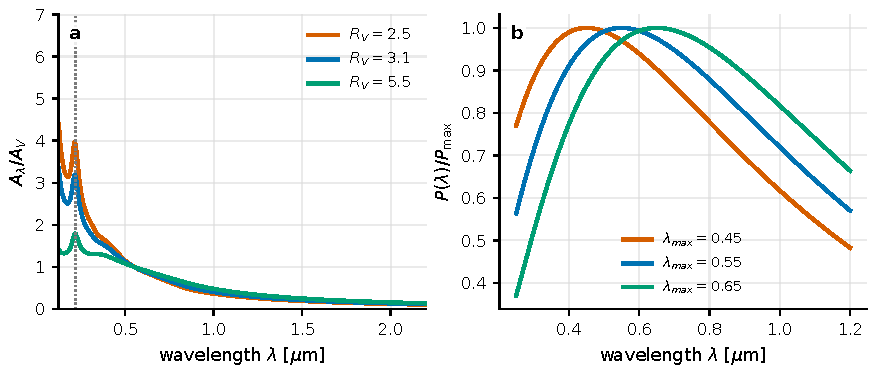
\includegraphics[width=0.94\linewidth]{figures/generated/chapter_14/ch14_dust_extinction_polarization.pdf}
\caption{Dust simultaneously changes a photon's flux, color, and polarization. The left panel is the CCM mean extinction curve; the larger \(R_V\), the ``grayer'' from optical to near-infrared; the ultraviolet bump near \(0.2175\,\mu{\rm m}\) is an important diagnostic of small grains and carbonaceous material. The right panel is the Serkowski polarization curve; the shift of the peak position \(\lambda_{\max}\) reflects changes in grain size and the alignment environment.}
\label{fig:e21-dust}
\end{figure}

\section{Gravitational lensing: turning one path into many}
\label{sec:e21-lensing}

The previous three rewriters all came from real media: electrons, magnetic fields, dust grains. The last one is different: gravitational lensing comes from \textbf{curved spacetime} itself. It does not change the frequency of a photon (no dispersion), but it changes the path, direction, and arrival time of the light. For the event table, the core action of a lens can be summarized in one sentence: \textbf{one source event can become multiple images, multiple arrival times, and multiple magnification weights}.

In the thin-lens approximation, the source's true direction and the image directions we see are connected by the lens equation:
\begin{equation}
  {\boldsymbol\beta}
  =
  {\boldsymbol\theta}
  -
  {\boldsymbol\alpha}({\boldsymbol\theta}),
  \label{eq:e21-lens-equation}
\end{equation}
\begin{formulaexplain}
\({\boldsymbol\beta}\) is the true angular position of the source, \({\boldsymbol\theta}\) is the angular position of the image, and \({\boldsymbol\alpha}\) is the reduced deflection angle, all in angular units (rad or arcsec). The equation says: the image direction \({\boldsymbol\theta}\) we see equals the true direction \({\boldsymbol\beta}\) plus the angle by which the mass bends the light. Given \({\boldsymbol\beta}\), this equation can have \textbf{multiple} solutions \({\boldsymbol\theta}\): those are the multiple images.
\end{formulaexplain}
The natural angular scale of the deflection is given by the Einstein angle. For a point-mass lens,
\begin{equation}
  \theta_E
  =
  \left(
  \frac{4GM}{c^2}
  \frac{D_{ls}}{D_lD_s}
  \right)^{1/2}.
  \label{eq:e21-einstein-angle}
\end{equation}
\begin{formulaexplain}
\(\theta_E\) is the Einstein angle, \(M\) is the lens mass, \(G\) is the gravitational constant, and \(D_l,D_s,D_{ls}\) are the angular diameter distances from observer to lens, to source, and from lens to source, respectively. The core factor \(4GM/c^2\) is the signature of general-relativistic light deflection (twice the Newtonian prediction). \(\theta_E\) sets the natural scale of the multiple-image separation and of microlensing.
\end{formulaexplain}
Two real orders of magnitude separate the two kinds of lensing. \(M=1\,M_\odot\), on Galactic-scale geometry, gives a \(\theta_E\) of order milliarcseconds (mas), too small to separate two images, so one can only see brightness fluctuating with time; this is \textbf{microlensing}: a foreground star drifting in front of a background star, magnifying it briefly. And a galaxy lens of \(M\sim10^{11}\text{--}10^{12}\,M_\odot\) gives a \(\theta_E\) of order arcseconds (arcsec), with the multiple images cleanly separated; this is \textbf{strong lensing}. The magnification is determined by the Jacobian determinant of the mapping from the image plane to the source plane:
\begin{equation}
  \mu
  =
  \frac{1}{\det\!\left(\partial{\boldsymbol\beta}/\partial{\boldsymbol\theta}\right)}.
  \label{eq:e21-magnification}
\end{equation}
\begin{formulaexplain}
\(\mu\) is the magnification, and the denominator is the Jacobian determinant from the image plane \({\boldsymbol\theta}\) to the source plane \({\boldsymbol\beta}\). The lens neither creates nor absorbs photons; it merely redistributes solid angle, so by whatever factor the area is stretched, that is how much the brightness is magnified. When the determinant tends to zero, the image plane is stretched infinitely and the magnification diverges: that curve is called a caustic.
\end{formulaexplain}
Near a caustic \(|\mu|\) can be very large (in theory divergent), but the finite source size, microlensing, dust, and time sampling all push down the peak magnification actually observable. The physics of this expression is very clean: magnification is a geometric redistribution, not a creation of energy out of nothing.

Now to the deepest, and most on-theme, point of lensing: the \textbf{time delay}. The different images travel paths of different length and pass through gravitational potentials of different depth, so their light does not arrive simultaneously. The arrival time is governed by the Fermat potential:
\begin{equation}
  t({\boldsymbol\theta},{\boldsymbol\beta})
  =
  \frac{D_{\Delta t}}{c}
  \left[
  \frac{1}{2}\,|{\boldsymbol\theta}-{\boldsymbol\beta}|^2
  -
  \psi({\boldsymbol\theta})
  \right],
  \qquad
  D_{\Delta t}
  =
  (1+z_l)\frac{D_lD_s}{D_{ls}} .
  \label{eq:e21-fermat-delay}
\end{equation}
\begin{formulaexplain}
\(t\) is the relative arrival time, the first term in the brackets \(\tfrac12|{\boldsymbol\theta}-{\boldsymbol\beta}|^2\) is the \textbf{geometric path difference} (the extra time spent taking a detour), and the second term \(\psi\) is the \textbf{gravitational potential delay} (the Shapiro delay, light ``travels more slowly'' in a deep potential well). \(D_{\Delta t}\) is the time-delay distance, and \(z_l\) is the lens redshift. The real images appear at the \textbf{stationary points} (minimum, maximum, or saddle) of this time surface, this is precisely Fermat's principle: ``light takes the path of extremal time.''
\end{formulaexplain}
The geometric origin of the time delay is hidden in the tug-of-war between these two terms: the farther one deviates from the source direction, the larger the geometric term (arriving late), but usually the closer to the mass and the deeper the potential well (the Shapiro term is also changing). The observed delay of two images is precisely the difference of their Fermat potentials:
\begin{equation}
  \Delta t_{AB}
  =
  \frac{D_{\Delta t}}{c}\,
  \Delta\phi_{AB}.
  \label{eq:e21-time-delay-distance}
\end{equation}
\begin{formulaexplain}
\(\Delta t_{AB}\) is the arrival-time difference between image \(A\) and image \(B\), and \(\Delta\phi_{AB}\) is the Fermat-potential difference of the two (computed from the lens mass model). Measuring \(\Delta t_{AB}\), and having a lens model that gives \(\Delta\phi_{AB}\), one can invert for \(D_{\Delta t}\), and since \(D_{\Delta t}\propto 1/H_0\), the time delay directly measures the Hubble constant.
\end{formulaexplain}
Order of magnitude: the \(\Delta t_{AB}\) of galaxy strong lensing is often days to months, and in a few cases up to years. Note that it is only about \(10^{-11}\) of \(D_{\Delta t}/c\) (because \(\Delta\phi_{AB}\) is a small number), so every bit of error in the lens potential, the external convergence, the mass-sheet degeneracy, and the light-curve sampling flows straight into the error budget of \(H_0\). Refsdal pointed out as early as 1964 that the time delay of multiple images can measure \(H_0\); modern time-delay cosmography, relying on multi-year monitoring, high-resolution imaging, lens-galaxy velocity dispersion, and environment modeling, has turned this idea into a measurement of \(H_0\) independent of the cosmic microwave background \citep{1964MNRAS.128..295R,1964MNRAS.128..307R,1986ApJ...310..568B,2016A&ARv..24...11T}. This is yet another beautiful encoding of the chapter: the time delay was originally the contamination of ``the same source copied into several time-offset replicas,'' and it turns out the expansion rate of the universe is locked in that time offset.

\begin{figure}[tbp]
\centering
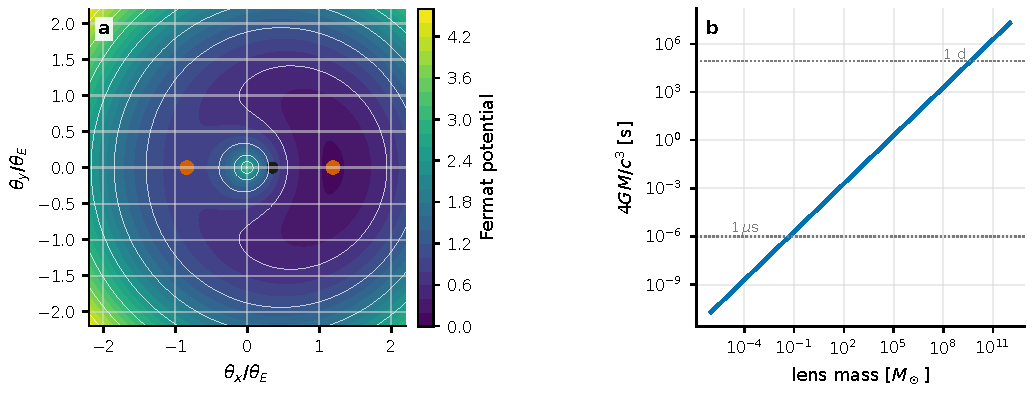
\includegraphics[width=0.94\linewidth]{figures/generated/chapter_14/ch14_lensing_time_delay.pdf}
\caption{The two scales of strong lensing. The left panel is the Fermat arrival-time surface of a point-mass lens, with the black dot the source position and the two orange dots the image positions; the images appear precisely at the stationary points of the arrival-time surface (minimum and saddle). The right panel gives the basic delay scale \(4GM/c^3\): stellar-mass lenses fall in microseconds to milliseconds, and galaxy and cluster lenses naturally enter the day-to-year time domain.}
\label{fig:e21-lensing}
\end{figure}

\paragraph{When wavelength cannot be ignored: from rays to diffraction}
\label{sec:e21-wavelensing}

The above treated light as ``rays,'' by default assuming that multiple paths can be cleanly separated. But when the wavelength is comparable to the time delay induced by the lens, geometric optics fails, and one must return to the \textbf{wave} picture, just as Chapter~\ref{chap:e02} repeatedly stressed, waves diffract and interfere. The criterion is a dimensionless frequency:
\begin{equation}
  w
  =
  \frac{8\pi GM(1+z_l)f}{c^3}.
  \label{eq:e21-wave-lensing-w}
\end{equation}
\begin{formulaexplain}
\(w\) is the dimensionless frequency of wave lensing, \(M\) is the lens mass, \(f\) is the wave frequency, and \(z_l\) is the lens redshift. \(w\) compares the wave period \(1/f\) with the time-delay scale \(\sim GM/c^3\) induced by the lens: when \(w\gg1\) the delay is far longer than the period and one returns to geometric optics; when \(w\lesssim1\) the delay is less than one period and diffraction cannot be neglected.
\end{formulaexplain}
In the geometric regime (\(w\gg1\)), multiple images can be separated and can coherently interfere like a double slit; in the diffraction regime (\(w\lesssim1\)), the caustics are smeared out and the magnification can no longer simply add the geometric images. The frequency-domain waveform is written as
\begin{equation}
  \tilde h_L(f)=F(f)\,\tilde h(f),
  \label{eq:e21-wave-amplification}
\end{equation}
\begin{formulaexplain}
\(\tilde h(f)\) is the unlensed frequency-domain waveform, \(\tilde h_L(f)\) is the lensed one, and \(F(f)\) is the complex amplification factor. It is a complex number, so it simultaneously carries \textbf{amplitude magnification} (modulus) and \textbf{phase delay} (argument), able to create frequency-dependent interference fringes.
\end{formulaexplain}
If the two paths have a delay \(\Delta t\), the two complex amplitudes add, and the beating with frequency gives a frequency-domain fringe spacing
\begin{equation}
  \Delta f \simeq \frac{1}{\Delta t}.
  \label{eq:e21-lensing-fringe-spacing}
\end{equation}
\begin{formulaexplain}
\(\Delta f\) is the spacing of the frequency-domain interference fringes, and \(\Delta t\) is the time delay of the two paths. This is yet another appearance of that old Fourier rule (Chapter~\ref{chap:e02}): two replicas separated in time by \(\Delta t\) weave, in the spectrum, fringes of spacing \(1/\Delta t\). The longer the path delay, the denser the frequency-domain oscillation.
\end{formulaexplain}
Plugging in numbers: \(\Delta t=2\,{\rm ms}\) gives a fringe spacing of \(\Delta f\approx500\,{\rm Hz}\). For the electromagnetic-wave frequencies of the optical and radio, \(f\sim10^{14}\) or \(10^{9}\,{\rm Hz}\), the \(w\) of an ordinary stellar- or galaxy-mass lens is astonishingly large, and geometric optics is almost perfect; but for gravitational waves in the LISA band (\(f\sim10^{-3}\,{\rm Hz}\)) with a lens of \(10^{6}\text{--}10^{9}\,M_\odot\), the wave-optics effect of \(w\sim1\) really does fall into the observing band \citep{2003ApJ...595.1039T}. This is the most direct interface between lensing and the quantum-optics through-line of this book: the interference after lensing is essentially the coherent superposition of the same source field along two paths, and what is read is still the phase.

\begin{figure}[tbp]
\centering
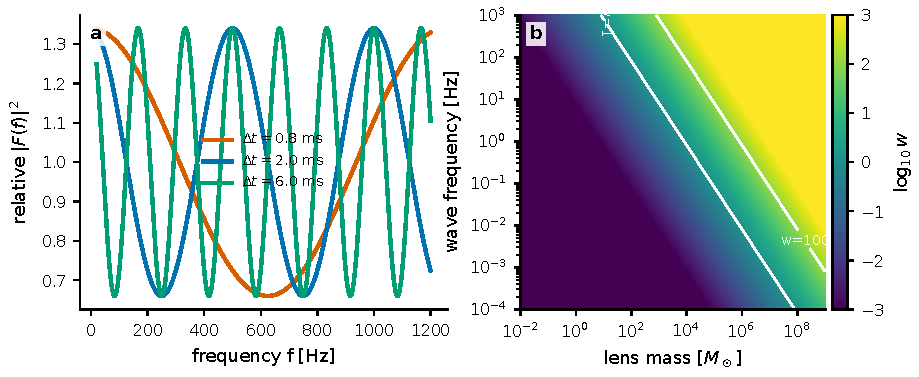
\includegraphics[width=0.94\linewidth]{figures/generated/chapter_14/ch14_wave_lensing_interference.pdf}
\caption{Wave-optics lensing transcribes the time delay into frequency-domain fringes. The left panel plots the oscillation of the relative amplification factor under different path delays, with fringe spacing \(\Delta f\simeq1/\Delta t\). The right panel gives the order of magnitude of \(w=8\pi GMf/c^3\); the region near the white line \(w=1\) is the transition between diffraction and geometric optics, and for \(w\gtrsim100\) one can usually treat the images as independent paths.}
\label{fig:e21-wave-lensing}
\end{figure}

\section{Contamination or encoding: what propagation means for coherence and timing}
\label{sec:e21-correlation}

Having gone around a full circle, we return to the book's through-line: the correlation function. The previous sections all rewrote the \textbf{labels of individual events}; this section looks at how they rewrite the \textbf{correlation between events}. The core insight is simple: multipath propagation (scattering, lensing) reshuffles the intensity correlation, because the two fluctuations observed need not come from the same source-end instant: they may be two replicas of the same source-end structure, arriving time-offset along different paths.

Writing the resolvable multipath as a string of delta impulse responses:
\begin{equation}
  h(t)=\sum_i \sqrt{\mu_i}\,e^{i\varphi_i}\,\delta(t-t_i),
  \label{eq:e21-multipath-impulse}
\end{equation}
\begin{formulaexplain}
\(h(t)\) is the multipath impulse response, \(\mu_i\) is the magnification of the \(i\)-th path, \(\varphi_i\) is its phase, and \(t_i\) is its arrival delay. Each delta function is a resolvable path: it is the concrete form of the abstract \(h_{ij}\) in Equation~\eqref{eq:e21-channel-time} in the ``discrete multiple-image'' case.
\end{formulaexplain}
If the phases \(\varphi_i\) are averaged out over the observing bandwidth or the source size (the common situation when coherence is diluted), the observed intensity is the sum of the path intensities weighted by magnification and offset in time:
\begin{equation}
  I_{\rm obs}(t)
  =
  \sum_i \mu_i\,I_{\rm src}(t-t_i).
  \label{eq:e21-multipath-intensity}
\end{equation}
\begin{formulaexplain}
\(I_{\rm obs}\) is the observed intensity, and \(I_{\rm src}\) is the source-end intensity. After the phase is averaged, the interference terms vanish, leaving only the sum of the path intensities weighted by \(\mu_i\), so one change at the source is repeated once at each of several different delays \(t_i\).
\end{formulaexplain}
Autocorrelating the intensity fluctuation \(\delta I=I-\langle I\rangle\), one can see how the ``echo'' enters the correlation function:
\begin{equation}
  C_{\rm obs}(\tau)
  =
  \left\langle
  \delta I_{\rm obs}(t)\,
  \delta I_{\rm obs}(t+\tau)
  \right\rangle
  =
  \sum_{ij}\mu_i\mu_j\,
  C_{\rm src}\!\left(\tau+t_i-t_j\right).
  \label{eq:e21-correlation-echo}
\end{equation}
\begin{formulaexplain}
\(C_{\rm obs}\) is the observed intensity autocorrelation, and \(C_{\rm src}\) is the source-end autocorrelation. The double sum means that \textbf{every pair of paths} contributes a correlation echo, the echo appearing at \(\tau=t_j-t_i\) with weight \(\mu_i\mu_j\). One peak originally is copied into a comb of echo peaks.
\end{formulaexplain}
This expression makes clear the effect of propagation on the intensity-correlation toolkit of Chapter~\ref{chap:e08}: \textbf{a correlation peak no longer uniquely corresponds to source-end physics}. The \(g^{(2)}(0)\) peak of thermal light, the microstructure of pulsar giant pulses, the narrowband scintillation of FRBs, and the delay of lensed multiple images can all fall into this framework, but their coherence times, bandwidths, and statistical distributions are each different. Seeing a single correlation peak is not enough to determine its physical origin. The prerequisites for using Equation~\eqref{eq:e21-correlation-echo} are hard: the source itself must have measurable fast structure, the propagation path must be stable, the observing time must be long enough, and the background and selection function must have been modeled. This is precisely the payoff of the ``channel with memory'' viewpoint: it forces you, before interpreting any correlation peak, to first ask, ``could this be just a late-arriving path?''

Propagation effects also delimit a class of quantum-foundations experiments. The so-called cosmic Bell test uses entangled photon pairs to make measurements at two stations, each side choosing measurement settings \(a,a'\) and \(b,b'\), and constructs the CHSH combination:
\begin{equation}
  S
  =
  E(a,b)+E(a,b')+E(a',b)-E(a',b'),
  \qquad
  |S|\le 2 .
  \label{eq:e21-chsh}
\end{equation}
\begin{formulaexplain}
\(S\) is the CHSH combination, and \(E(a,b)\) is the correlation expectation of the two stations' measurement results under given settings. Local hidden-variable theories require \(|S|\le2\); quantum mechanics can violate it up to \(2\sqrt2\). The distinctive feature of a cosmic Bell experiment is using \textbf{astronomical photons} to decide the settings \(a,b\) in real time.
\end{formulaexplain}
Its point is not that the celestial photons themselves are in an entangled state, but to use the light of distant celestial objects to \textbf{choose the measurement settings in real time}: the Galactic-star version uses starlight color to generate \(a,b\), pushing the possible ``common cause'' back to hundreds or thousands of years ago; the quasar version is even more extreme, pushing the common past of the freedom-of-choice loophole back to the early universe \citep{2017PhRvL.118f0401H,2018PhRvL.121h0403R} (Figure~\ref{fig:e21-cosmic-bell}). And this requires everything in this chapter: the arrival time of the starlight must have the atmospheric delay subtracted (the time synchronization of Chapter~\ref{chap:e13}), the color must have the dust reddening subtracted, radio quasars must also account for dispersion and scattering, and the instrumental electronic delay must enter the experimental timing term by term: every absorption, reddening, dispersion, and delay in propagation must be placed into the experiment's causal timing, otherwise the loophole cannot be sealed tight.

\begin{figure}[tbp]
\centering
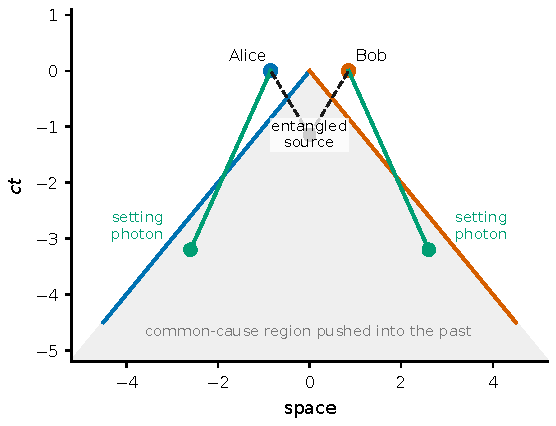
\includegraphics[width=0.72\linewidth]{figures/generated/chapter_14/ch14_cosmic_bell_lightcones.pdf}
\caption{The light-cone structure of a cosmic Bell experiment. The entangled source emits photon pairs in the local experiment, and the measurement settings of Alice and Bob are decided in real time by photons from distant stars or quasars; the earlier the emission events of these setting photons and the greater their directional separation, the larger the spacetime region from which a ``common cause'' can be excluded (the gray region in the figure). A real experiment must also add, term by term, atmospheric propagation, dust reddening, detector response, and electronic delay. This is precisely where each effect of this chapter must enter the experimental timing.}
\label{fig:e21-cosmic-bell}
\end{figure}

Finally, let us regard these ``ordinary'' propagation effects as the \textbf{error floor} of new-physics searches. Axion-like particles can let photons convert in a magnetic field and cause spectral absorption, cosmic birefringence rotates polarization, and dark-matter substructure can rewrite the magnification and time delay of a lens. All these fascinating explanations must first be compared with plasma dispersion, dust, conventional lensing, and instrumental terms within the same model. Only when a residual signal simultaneously withstands the four tests of time, frequency, polarization, and angular position, and no known propagation effect can subtract it away, does it qualify to queue up as a candidate for new physics. This is the most practical conclusion of the chapter's theme ``contamination is background, encoding is signal'': first characterize this channel with memory to the end, and what remains is what truly belongs to the source, and even to new physics.

\section*{Chapter Summary}
\addcontentsline{toc}{section}{Chapter Summary}

\begin{itemize}
\item \textbf{Propagation is a channel with memory, not gray glass.} Equation~\eqref{eq:e21-channel-time} writes the source-end field to detector event as a convolution: the medium rewrites each photon's time, frequency, polarization, and direction label, not merely multiplies by a constant.
\item \textbf{The \(\nu^{-2}\) law of dispersion is derived step by step from the group velocity.} Refractive index \(\to\) group velocity \(v_g\approx c(1-\omega_p^2/2\omega^2)\) \(\to\) integration along the line of sight, giving \(\Delta t\propto{\rm DM}/\nu^2\) (Equation~\eqref{eq:e21-dm-delay}). The root cause of low frequency arriving late is ``the low-frequency group velocity is slower.'' DM is the electron column density, and the DM--redshift relation of FRBs can weigh the cosmic baryons.
\item \textbf{Faraday rotation adds the magnetic-field direction to dispersion.} The slope of the polarization angle against \(\lambda^2\) is RM, whose integrand \(n_e B_\parallel\) is signed, so RM/DM gives the electron-weighted mean magnetic field (Equation~\eqref{eq:e21-bfield-rm-dm}), but only when the two are cospatial does it have direct physical meaning.
\item \textbf{Scattering scrambles coherence, and also offers ultra-high resolution for free.} A one-sided exponential kernel drags a narrow pulse into a long tail (\(\tau_{\rm sc}\propto\nu^{-4}\)), and the decorrelation bandwidth \(\Delta\nu_d\simeq1/2\pi\tau_{\rm sc}\) (Equation~\eqref{eq:e21-decorrelation-bandwidth}) determines whether broadband coherent superposition is diluted; under weak scattering, scintillation can conversely be inverted for the screen velocity, screen distance, and source angular size.
\item \textbf{Dust is a loss channel with wavelength selectivity.} Extinction \(F_{\rm obs}=F_{\rm int}10^{-0.4A_\lambda}\) makes the source both dimmer and redder, and \(R_V\) sets the grayness of the curve; the residual of the mean extinction law is the dominant systematic of polarization and the early SED; Serkowski polarization and dust light echoes are both foregrounds that must be subtracted first.
\item \textbf{Gravitational lensing turns one path into many.} The Einstein angle sets the scale (stellar mass mas, galaxy arcsec), the magnification is the reciprocal of the geometric Jacobian, and the time delay is determined by the geometric term plus the Shapiro term of the Fermat potential (Equation~\eqref{eq:e21-fermat-delay}), and it measures the Hubble constant because \(D_{\Delta t}\propto1/H_0\). When wavelength cannot be ignored, use the dimensionless frequency \(w\) to judge the geometric/diffraction regime.
\item \textbf{Contamination is encoding.} Multipath copies one source-end fluctuation into a correlation echo (Equation~\eqref{eq:e21-correlation-echo}), so a correlation peak does not uniquely correspond to source-end physics; these ordinary effects in turn constitute the timing constraints of the cosmic Bell test and the error floor of new-physics searches.
\end{itemize}

\medskip
\noindent\textbf{Questions to Ponder.}
\begin{itemize}
\item If an FRB is measured to have a delay of \(1.2\,{\rm s}\) between \(1.4\,{\rm GHz}\) and \(0.8\,{\rm GHz}\), roughly what is its DM? (Invert using Equation~\eqref{eq:e21-dispersion-delay}.) If this line of sight is mainly within the Galaxy, is it reasonable compared with the typical high-Galactic-latitude value?
\item For the same RM, if there is a field reversal along the line of sight, will the RM you measure be larger or smaller? Why is DM unaffected by this reversal?
\item The time delay of the two images of a galaxy strong lens is measured to be \(30\) days, and the lens model gives \(\Delta\phi_{AB}\). To measure \(H_0\) to 3\% precision, which links in Equation~\eqref{eq:e21-time-delay-distance} (light-curve sampling, external convergence, mass-sheet degeneracy) are most likely to become the bottleneck?
\end{itemize}
